\chapter{Theoretical Background}
\label{chap:two}

\section{Credit Risk}

\subsection{Regulation}

\textbf{TBD}

\section{Terminology}

\textbf{TBD}
\section{Algorithms}

In this section, several algorithms, which are used in the machine learning implementation, are going to be described. Since the goal is to predict whether or not given client will default, henceforth only (binary) classification algorithms as a part of the supervised learning are described. In other words, regression models and unsupervised learning algorithms are out of the scope of this thesis.
\subsection{Logistic Regression}

\textbf{TBD}

Despite the algorithm's name, it is actually not a regression but rather a classification model.
In contrast, a linear regression's target variable is continuous whereas regarding a logistic regression, the target variable is binary or dichotomous.
For the probability estimation it is using a logistic, or so-called sigmoid function, which maps any real value within the range of 0 to 1 and takes a S-shaped curve as can be seen in \autoref{fig:sigmoid}.

\begin{figure}[H]
    \centering
    \caption{Logistic function}\vspace{0.5em}
    \label{fig:sigmoid}\
    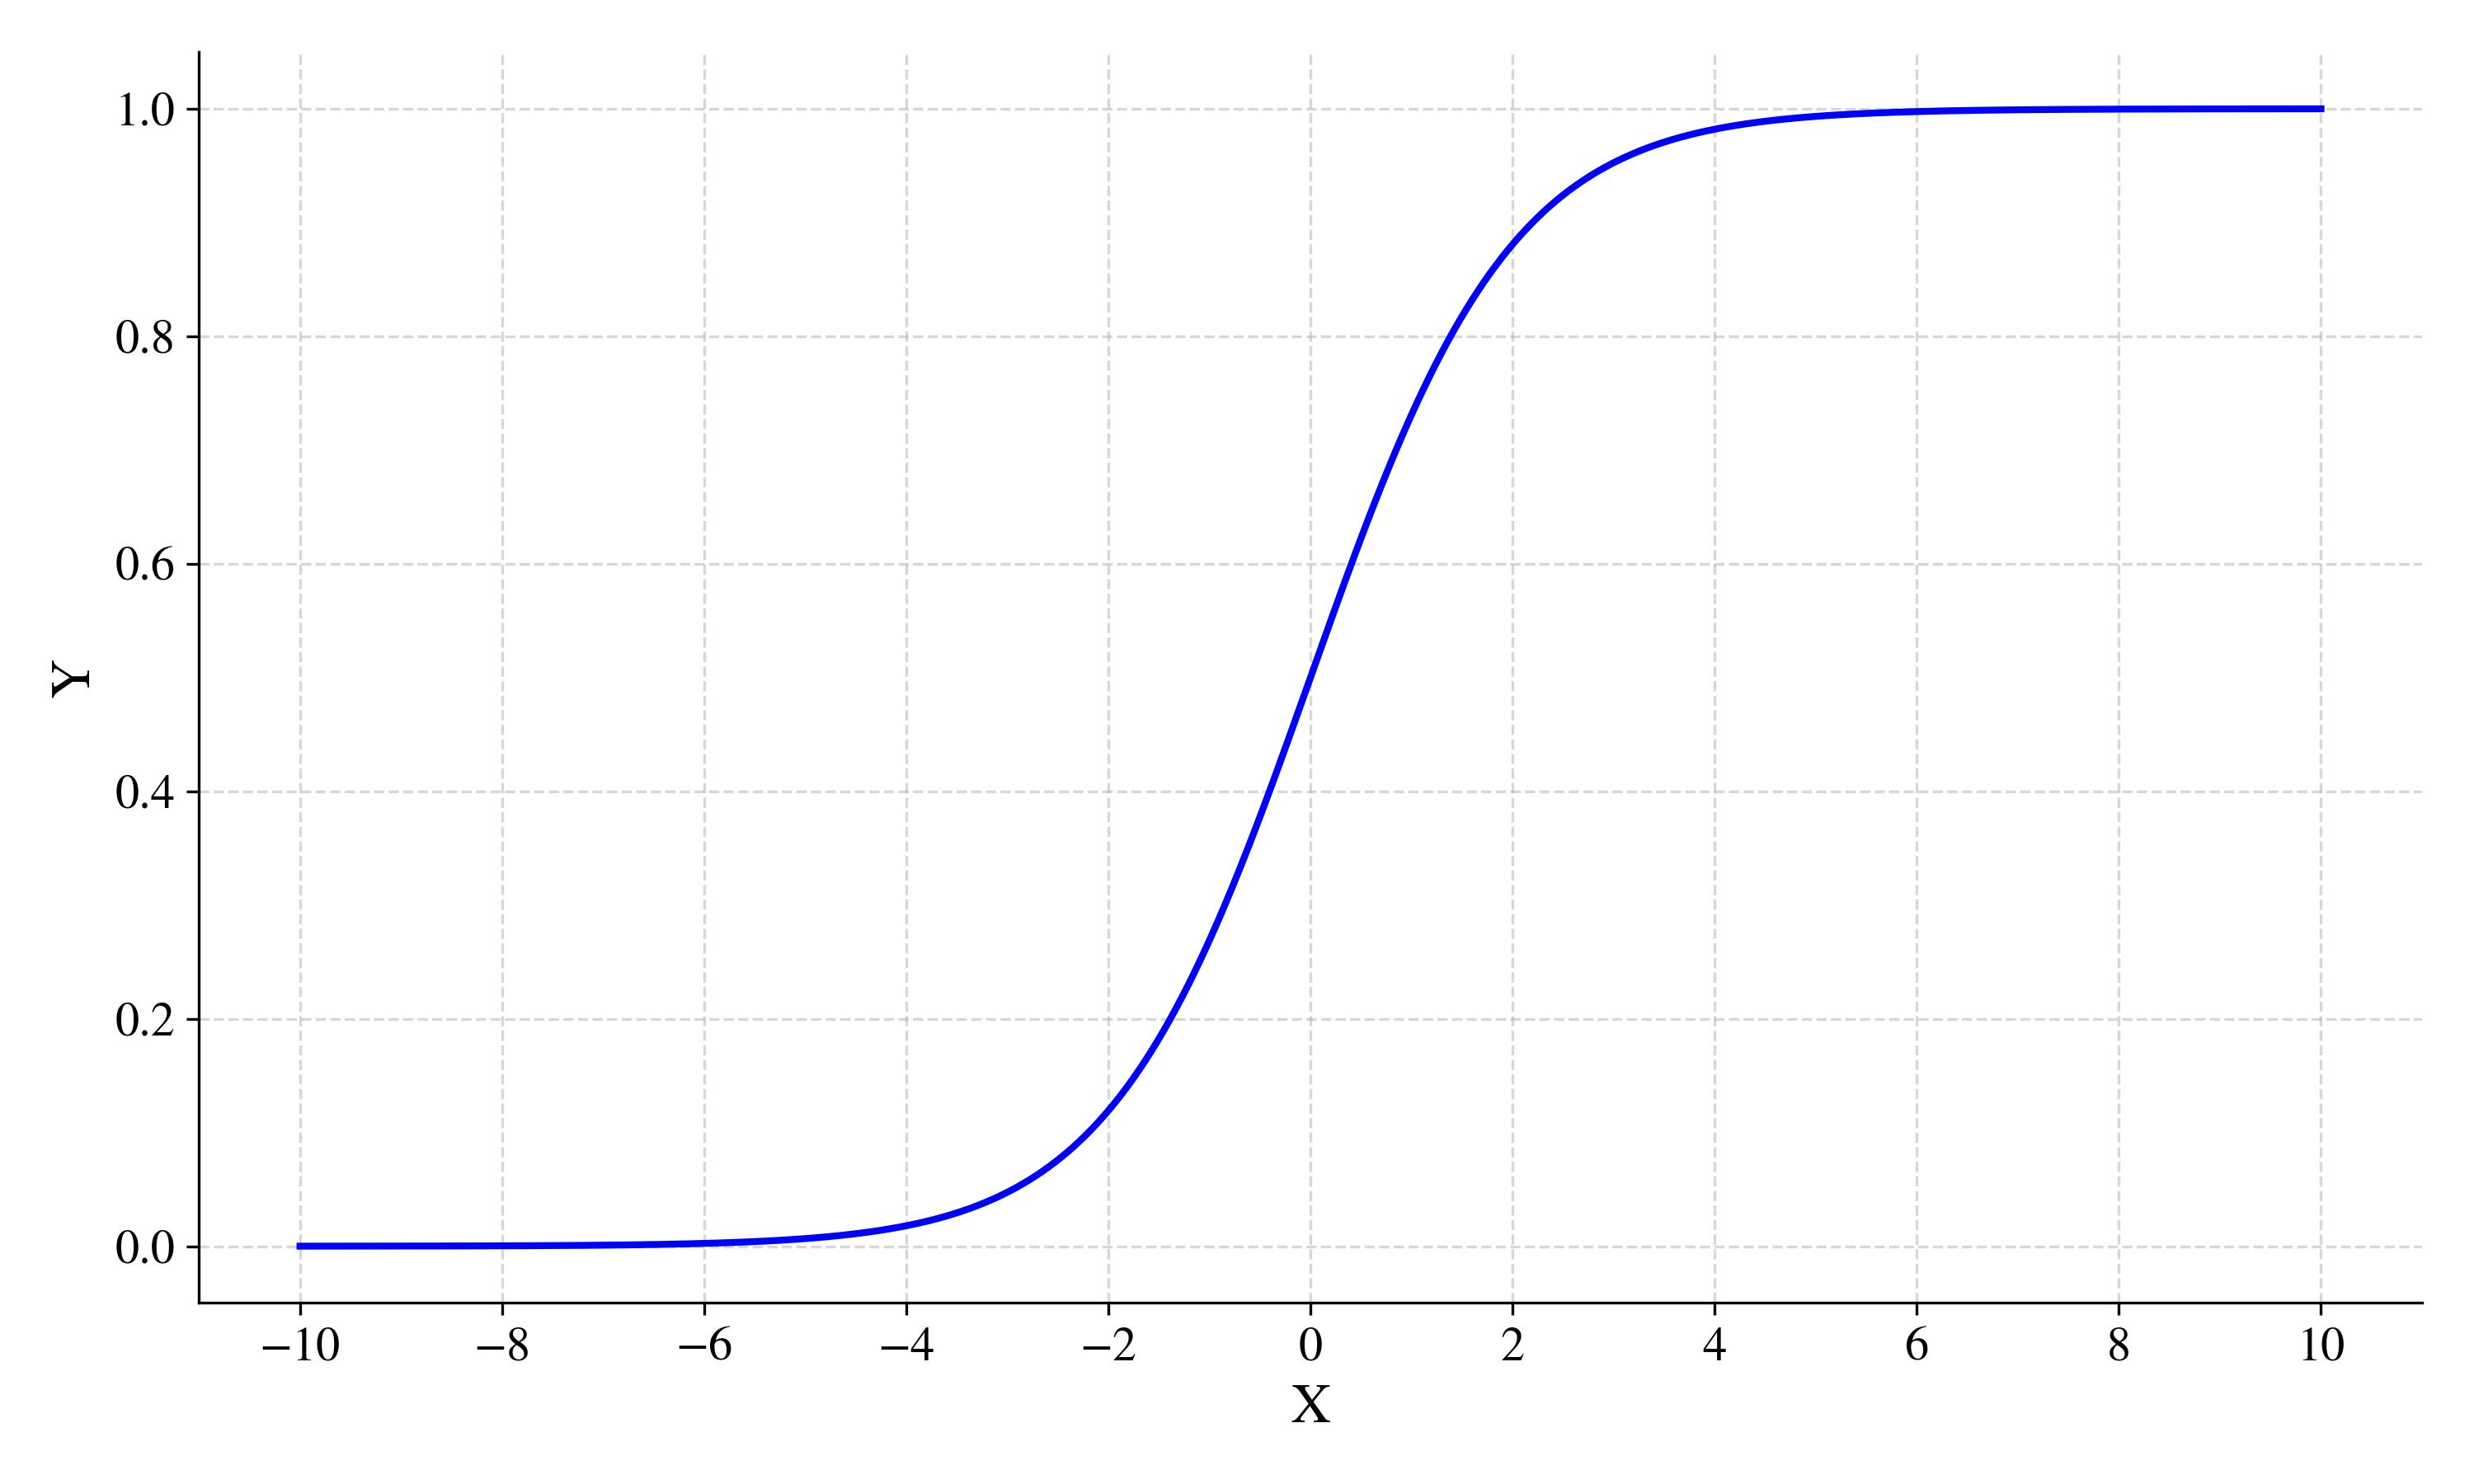
\includegraphics[width=130mm]{Figures/sigmoid.jpg}
    \centering{\begin{source}\citep{wendler2021data}\end{source}}\vspace{-1em}
\end{figure}

The linear form of the logistic regression with n features can be written as:

\begin{equation}\label{eq}
    \ln\left(\frac{P}{1-P}\right) = \beta_0  + \sum_{i=1}^{n} \beta_i X_i
\end{equation}

where $P$ is the probability of the occurred event, conditional on the set of given features. Let us denote $Y=1$ as an observed target instance where the event occurred (e.g., defaulted), then:
\begin{equation}\label{eq}
    P = \operatorname{Pr}(Y=1 \mid X_1,X_2,\ldots,X_n)
\end{equation}

Therefore, the term within the natural logarithm are the odds or more particularly, the ratio of the probability of the event with respect to the probability of non-event, both conditional on the same set of given features.
\begin{equation}\label{eq}
    \begin{aligned}
    \frac{P}{1-P}  {} & = \frac{\operatorname{Pr}(Y=1 \mid X_1,X_2,\ldots,X_n)}{1-\operatorname{Pr}(Y=1 \mid X_1,X_2,\ldots,X_n)} \\
    & = \frac{\operatorname{Pr}(Y=1 \mid X_1,X_2,\ldots,X_n)}{\operatorname{Pr}(Y=0 \mid X_1,X_2,\ldots,X_n)}
\end{aligned}
    \end{equation}

Referring to the previous equations, solving for $P$, henceforth we get a final equation for computing the probability of occurred event with usage of logistic regression:

\begin{equation}\label{eq}
P = \frac{1}{1+e^{-\left(\beta_0 + \displaystyle\sum_{i=1}^{n} \beta_i X_i\right)}}
\end{equation}

\subsection{Decision Tree}

\textbf{TBD}
\subsection{Naive Bayes}

\textbf{TBD}

Naive Bayes is a classification and probabilistic machine learning algorithm which is based on the Bayes theorem:

\begin{equation}\label{eq}
    \operatorname{Pr}\left(C=c \mid E \right) = \frac{\operatorname{Pr}\left(C=c\right) \times \operatorname{Pr}\left(E \mid C=c\right)}{\operatorname{Pr}\left(E\right)}
\end{equation}

where:
\begin{itemize}\setlength\itemsep{0em}
	\item $\operatorname{Pr}\left(C=c \mid E \right)$ is the posterior probability which is the probability that the target variable $C$ takes on the class of interest $c$ after taking the evidence $E$.
	\item $\operatorname{Pr}\left(C=c\right)$  is the prior probability of the class $c$ is the probability we would assign to the class $c$ before seeing any evidence $E$.
	\item $\operatorname{Pr}\left(E \mid C=c\right)$ is the probability of seeing the evidence $E$ conditional on the given class $c$.
	\item $\operatorname{Pr}\left(E\right)$ is the probability of the evidence $E$.
\end{itemize}

With regards to the binary classification, we can substitute $Y$ as a target variable instead $C$, and set of features $X$ which will refer to the set of evidence $E$.
Assuming that $Y=1$ refers to the occurrence of given event (e.g., default), henceforth the probability of default using the Naïve Bayes algorithm can be mathematically expressed as:

\begin{equation}\label{eq}
    \operatorname{Pr}\left(Y=1 \mid X \right) = \frac{\operatorname{Pr}\left(Y=1\right) \times \operatorname{Pr}\left(X \mid Y=1 \right)}{\operatorname{Pr}\left(X\right)}
\end{equation}

One of the assumptions of this algorithm is the conditional probabilistic independence among the features.
Therefore, instead of computing the probability of all features together, conditional on the class event, for each feature $X$ we will compute its probability, conditional on the class event. Hence:

\begin{equation}\label{eq}
    \operatorname{Pr}\left(Y=1 \mid X \right) = \prod_{i=1}^{n} \operatorname{Pr}\left(X_i \mid Y=1\right)
\end{equation}

With regards to the conditional independence, we can also derived the probability of evidence $E$ or set of features $X$ respectively, as a sum of the probability of given set of features, conditional on class one (event), and of the probability of given set of features, conditional on one class two (non-event).
Therefore:
\begin{equation}\label{eq}
\operatorname{Pr}\left(X\right) = \operatorname{Pr}\left(X \mid Y=1\right) \times \operatorname{Pr}\left(Y=1\right) + \operatorname{Pr}\left(X \mid Y=0\right) \times \operatorname{Pr}\left(Y=0\right)
\end{equation}
Therefore:
\begin{equation}\label{eq}
    \begin{aligned}
    \operatorname{Pr}\left(X\right) = {} & \prod_{i=1}^{n} \operatorname{Pr}\left(X_i \mid Y=1\right) \times \operatorname{Pr}\left(Y=1\right) + \\
    & \prod_{i=1}^{n} \operatorname{Pr}\left(X_i \mid Y=0\right) \times \operatorname{Pr}\left(Y=0\right)
    \end{aligned}
    \end{equation}
Finally, we can derive the final formula for Naïve Bayes the posterior probability as:

    \begin{equation}
        \frac{\displaystyle\prod_{i=1}^{n} \operatorname{Pr}(X_i \mid Y=1)}{\displaystyle\prod_{i=1}^{n} \operatorname{Pr}(X_i \mid Y=1) \operatorname{Pr}(Y=1) + \displaystyle\prod_{i=1}^{n} \operatorname{Pr}(X_i \mid Y=0) \operatorname{Pr}(Y=0)}
        \end{equation}


\subsection{K-Nearest Neighbors}

The goal of K-nearest Neighbors algorithm (also known as KNN) is to find $k$ instances that are most similar to particular instances y in the n-dimensional space, where n is the number of features.
The principle of this algorithm consists in the similarity between the instances as it assumes that the similar instances are close to each other.
Based on the predetermined $k$ neighbors, it will predict the class based on the k nearest instances.


There are several ways how to measure the distance. The most used one is the Euclidean distance. Geometrically, it is a straight line between the two points  and within two-dimensional space, it can be derived from the Pythagorean theorem, where the hypotenuse is the straight line measuring the distance. In the n-dimensional space, we take the sum the squared differences between the data points $x$ and $y$, underneath the square root in order to compute the total Euclidean distance.
\begin{equation}\label{eq}
d_{Euclidean}(x,y) = \sqrt{\sum\limits_{i=1}^{n} (x_i - y_i)^2}
\end{equation}

Other distance measure is the Manhattan distance measure, which is known as a city block distance, referring to the real-life problems, more particularly in order to reach particular destination, we have to take the path in between the blocks.
Mathematically, it is similar to the Euclidean distance, but instead of squared differences, it sums the absolute differences between the data points.
\begin{equation}\label{eq}
d_{Manhattan}(x,y) = \sqrt{\sum\limits_{i=1}^{n} |x_i - y_i|}
\end{equation}

The last measure is the Minkowski distance which is the generalized form Euclidean or Manhattan distance respectively.
It depends on p which represents the order of the norm. Hence, the Euclidean distance has the second order of the norm, whereas Manhattan distance has the first order of the norm.
\begin{equation}\label{eq}
d_{Minkowski}(x,y) = \sqrt[p]{\sum\limits_{i=1}^{n} |x_i - y_i|^p}
\end{equation}

Within the training process, KNN memorizes training instances and afterwards when it encounters a new instance, it tries to search for such training instance(s) which most strongly resembles the new instance \citep{witten2011data}.
Therefore, After the training process, when it comes to the prediction, the KNN compares the new instance to the training instances, calculates the distances between the the new input and the training instances, and predicts the class based on on the majority voting within the $k$ nearest neighbors, or predicts the probability scores as the fraction of positive instances within the $k$ nearest neighbors.


On the following \autoref{fig:knn-example}, let us consider 2--dimensional space and that $k$ is equal to 4, hence we are looking at four nearest neighbors for such new instance. Further, let us consider two classes - red squares and green triangles.
By looking at the four nearest neighbors, we can observe that three out of the nearest neighbors are the red triangles.
Therefore, when applying majority voting, KNN would predict such instance as a red triangle, or would predict a probability score of 0.75 for the red triangle.

\begin{figure}[H]
    \centering
    \caption{K-Nearest Neighbors with $k=4$}\vspace{0.5em}
    \label{fig:knn-example}\
    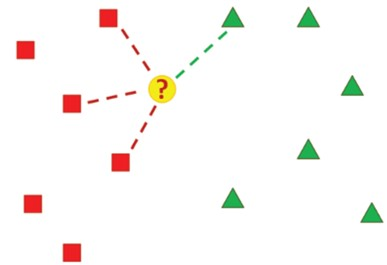
\includegraphics[width=80mm]{Figures/KNN_example.jpg}

    \centering{\begin{source}\citep{mucherino2009data}\end{source}}\vspace{-1em}
\end{figure}

\subsection{Random Forest}

ratatatat \citep{rigatti2017random}

\textbf{TBD}
\subsection{Gradient Boosting}

\textbf{TBD}
\subsection{Support Vector Machine}

\textbf{TBD}
\subsection{Neural Networks}

\textbf{TBD}

\section{Evaluation Metrics}

\textbf{TBD}

This section focuses on particular measures through which it is possible to determine a predictive power of model in terms of its performance.
The are many ways, how to evaluate the model's performance, therefore, only the most common ones and the most relevant are further described.
Note, since default prediction regards classification tasks, therefore regression's evaluation metrics are omitted.

\subsection{Confusion Matrix}

\textbf{TBD}

Confusion matrix is a table which summarizes the classification model's performance with respect to the actual classes and predicted classes.
It is a square $n \times n$ matrix, where $n$ determines number of classes within the target variable.
Let us denote the confusion matrix as $C\left(f\right)$ for classification algorithm $f$. 
Its elements can be denoted as $c_{i,j}$ where $i$ and $j$ refer to the row and column indices, respectively, or more particularly, $i$ refers to the actual class and $j$ to the class predicted by the classifier $f$.
Each element of the confusion matrix refers to the number of instances corresponding to actual class $i$ and predicted class $j$. For instance, the element $c_2,1$ would refer to the number of instances which have the actual class $2$ but have been classified as class $1$.
Mathematically, the confusion matrix can be written as following:

\begin{equation}\label{eq}
C = {c_{i,j} = \sum_{l=1}^{m}[(y_l=i) \land (f(x_l)=j)]}
\end{equation}

Or either in matrix form as:

\begin{equation}\label{eq}
    C_{i \times j} = \begin{bmatrix}
    c_{1,1} & c_{2,1} & \cdots & c_{1,j} \\
    c_{2,1} & c_{2,2} & \cdots & c_{2,j} \\
    \vdots & \vdots & \ddots & \vdots \\
    c_{i,1} & c_{i,2} & \cdots & c_{i,j} \\
    \end{bmatrix}
\end{equation}

From the given matrix, the diagonal elements represent the numbers of correctly classified instances, whereas the non-diagonal elements represent the numbers of misclassified instances.
Further, let us consider a binary classification - hence, the confusion matrix will have a form of $2\times 2$.

\begin{equation}
    C_{2 \times 2} = \begin{bmatrix}
    c_{1,1} & c_{1,2} \\
    c_{2,1} & c_{2,2} \\
    \end{bmatrix}
    \end{equation}


We can this rewrite confusion matrix as:

\begin{equation}
    C_{2 \times 2} = \begin{bmatrix}
    TP & FN \\
    FP & TN \\
    \end{bmatrix}
    \end{equation}

where:
\begin{itemize}\setlength\itemsep{0em}
    \item TP is the True Positive which refers to the number of instances which correspond to the actual class $True$ and indeed have been correctly classified as class $True$.
	\item $FP$ is the False Positive which refers to the number of instances which correspond to the actual class $True$, but have been incorrectly classified as class $False$. In the statistics and hypothesis--testing terms, it can be also called as Type 1 Error.
	\item $FN$ is the False Negative which refers to the number of instances which correspond to the actual class $False$, but have been incorrectly classified as class $True$. In the statistics and hypothesis--testing terms, it can be also called as Type 2 Error.
	\item $TN$ is the True Negative which refers to the number of instances which correspond to the actual class $False$ and indeed have been correctly classified as class $False$.
\end{itemize}

\subsection{Accuracy}

\textbf{TBD}

\begin{equation}\label{eq}
    Accuracy = \frac{TP + FN}{TP + TN + FP + FN}
\end{equation}

\subsection{Recall}

\textbf{TBD}

\begin{equation}\label{eq}
    Precision = \frac{TP}{TP + FN}
\end{equation}

\subsection{Precision}

\textbf{TBD}

\begin{equation}\label{eq}
    Precision = \frac{TP}{TP + FP}
\end{equation}

\subsection{F1 Score}

\textbf{TBD}

\begin{equation}\label{eq}
    F1 = \frac{2 \times Precision \times Recall}{Precision + Recall} = \frac{2 \times TP}{2 \times TP + FP + FN}
\end{equation}

\subsection{AUC}

\textbf{TBD}

In order to derive Area Under the Curve ($AUC$), first we need to define Receiver Operating Characteristics ($ROC$) curve.
ROC curve is two-dimensional visualization of the model performance as a probability curve in terms of True Positive Rate ($TPR$) and False Positive Rate ($FPR$) based on varying the given threshold.

Briefly, it can be construct as following: First, we need to sort the instances by the predicted probability and based on the given probability, we set a threshold - what will be above the threshold will be classified as $True$ instance and what is below the threshold will be classified as $False$ instance.
Based on these classified instances, the confusion matrix can be constructed and via which we can compute the $TPR$ and $FPR$ values.
Thus, if the probability is 1, the threshold will be 1 as well and hence:
\begin{itemize}\setlength\itemsep{0em}
    \item $TPR$ will be 0 because there is no probability which is higher than 1 and hence, everything will be classified as $False$ which will result into $TP$ of 0, and subsequently into $TPR$ of 0 as well.
	\item $FPR$ will be 0, too – since everything will be classified as $False$, therefore $FP$ will be 0 which implies $FPR$ to be 0, too.
\end{itemize}
On the other hand, if the probability is 0, the threshold will be 0 as well and hence:
\begin{itemize}\setlength\itemsep{0em}
    \item $TPR$ will be 1 because there is no probability which is lower than 0 and hence, everything will be classified as $True$ which will result into $FN$ of 0, and subsequently into $TPR$ of 1.
	\item $FPR$ will be 1, too – since everything will be classified as $True$, therefore $TN$ will be 0 which implies $FPR$ to be 1.
\end{itemize}

Thus, based on each threshold, the $TPR$ and $FPR$ will be to coordinates for single point within the graph and based on such points, we can construct the ROC curve.
Such visualization on the following \autoref{fig:roccurvetheory}.
Note the diagonal line represents a random model which randomly and correctly predicts the $True$ and $False$ classes in such way, that $FPR$ and $TPR$ are the same.
Logically, a decent model should perform better than the random model, thus it the ROC curve should be above the diagonal line.
Intuitively, the best possible theoretical model would have $TPR$ of 1 and $FPR$ of 0, meaning that all the $True$ actual classes should be predicted as $True$ and all the $False$ actual classes should not be classified as $True$
 Within the ROC curve, the given curve reaches the left top corner which corresponds to the coordinates of $TPR$ and $FPR$.

 \begin{figure}[H]
    \centering
    \caption{ROC Curve}\vspace{0.5em}
    \label{fig:roccurvetheory}\
    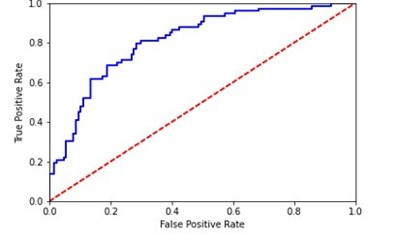
\includegraphics[width=100mm]{Figures/ROC_theory.jpg}

    \centering{\begin{source}Author's results in Python.\end{source}}\vspace{-1em}
\end{figure}

$AUC$ is basically the representation of ROC curve as a single number as it aggregates the performance on all possible thresholds.
$AUC$ can be interpreted as the probability that the randomly chosen actual $True$ instance is ranked higher than the randomly chosen actual $False$ instance.
Since ROC curve is a probability curve, thus it is considering distribution curve of $TP$ and distribution class of $TN$, separated by particular threshold – hence, $TP$ would have probability scores above the given thresholds, whereas $TN$ would have probability scores below the threshold.
If these curves do not overlap, meaning the model can perfectly distinguish between the $True$ and $False$ values, therefore the $AUC$ would be 1 and the ROC curve would reach the left top corner.
However, this idealistic situation does not occur in the practice at all, but rather the two distributions are overlapping since the misclassification of the classes takes the place.
The bigger overlap, the lower $AUC$ is.
If the distributions are completely overlapping, it implies the $AUC$ of 0.5, meaning that the model cannot distinguish between the $True$ and $False$ classes, which is the worst scenario.
On the other hand, if the distributions are totally opposite (meaning that the $TP$ instances would have probability scores below the given threshold, whereas the $TN$ instances would have probability scores above the given threshold), the $AUC$ would be 0 since the model is predicting the $True$ actual classes instead of $False$ and vice versa.

As the $AUC$ is an area present underneath the ROC curve, mathematically, it can be computed with the definite integral where $x$ is the given threshold:

\begin{equation}\label{eq}
    AUC = \int_{0}^{1} TPR \left(FPR^{-1}\left(x \right)\right) dx
\end{equation}

\subsection{Kolmogorov-Smirnov Distance}

\textbf{TBD}

\begin{equation}\label{eq}
    KS = \max_{x \in \mathbb{R}} \left| \hat{F}_n \left(x \right) - F \left(x \right) \right|
\end{equation}


\subsection{Somer's D}

\textbf{TBD}

\begin{equation}\label{eq}
    SD = \frac{\tau \left(X, Y\right)}{\sqrt{\tau \left(X, X\right) \tau \left(Y, Y\right)}}
\end{equation}


\subsection{Matthews Correlation Coefficient}

\textbf{TBD}

\begin{equation}\label{eq}
    MCC = \frac{TP \times TN - FP \times FN}{\sqrt{(TP + FP) (TP + FN) (TN + FP) (TN + FN)}}
\end{equation}


\subsection{Brier Score Loss}

\textbf{TBD}

\begin{equation}\label{eq}
    BSL = \frac{1}{n} \sum_{i=1}^{n} (y_i - \hat{y}_i)^2
\end{equation}


\subsection{Jaccard Score}

\textbf{TBD}

\begin{equation}\label{eq}
    JC = \frac{|y \cap \hat{y} |}{|y \cup \hat{y} |}
    \end{equation}


\subsection{Zero-One Loss}

\textbf{TBD}

\begin{equation}\label{eq}
    ZOL = \frac{1}{n} \sum_{i}^{n} \delta_{y_{i=1} \neq \hat{y}_{i}} \text{ , where } \delta_{y_{i} \neq \hat{y}_{i}} = \begin{cases}
        1, & \text{if $x<0$}.\\
        0, & \text{otherwise}.
      \end{cases}
\end{equation}
\section{Hyperparameter Tuning}

\textbf{TBD}
\subsection{Grid Search}

\textbf{TBD}
\subsection{Random Search}

\textbf{TBD}
\subsection{Bayesian Optimization}

\textbf{TBD}
\section{Imbalanced Class Distribution}

\textbf{TBD}
\subsection{Random Oversampling}

\textbf{TBD}
\subsection{SMOTE Oversampling}

\textbf{TBD}
\subsection{ADASYN Oversampling}

\textbf{TBD}
\section{Optimal Binning}

\textbf{TBD}
\subsection{Weight of Evidence Encoding}

\textbf{TBD}